
\section{Figures}
\begin{figure}
    \centering
    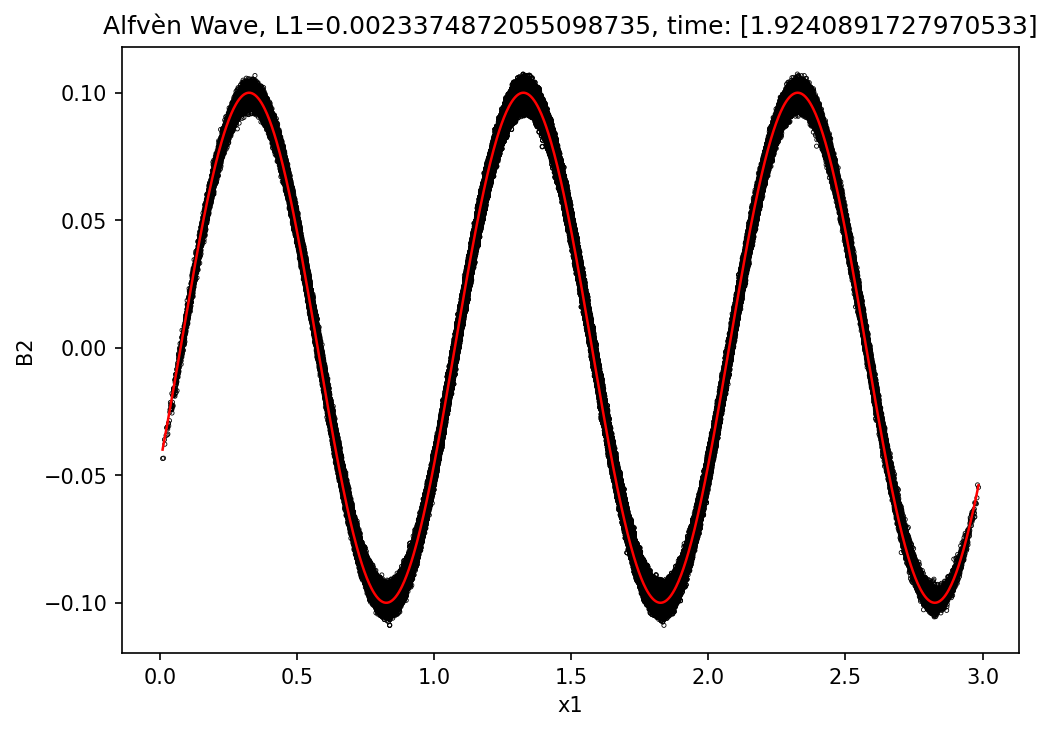
\includegraphics[width=0.5\linewidth]{img/Alfven/alfven_wave.png}
    \caption{Alfven Wave}
    \label{fig:placeholder}
\end{figure}

\begin{figure}
    \centering
    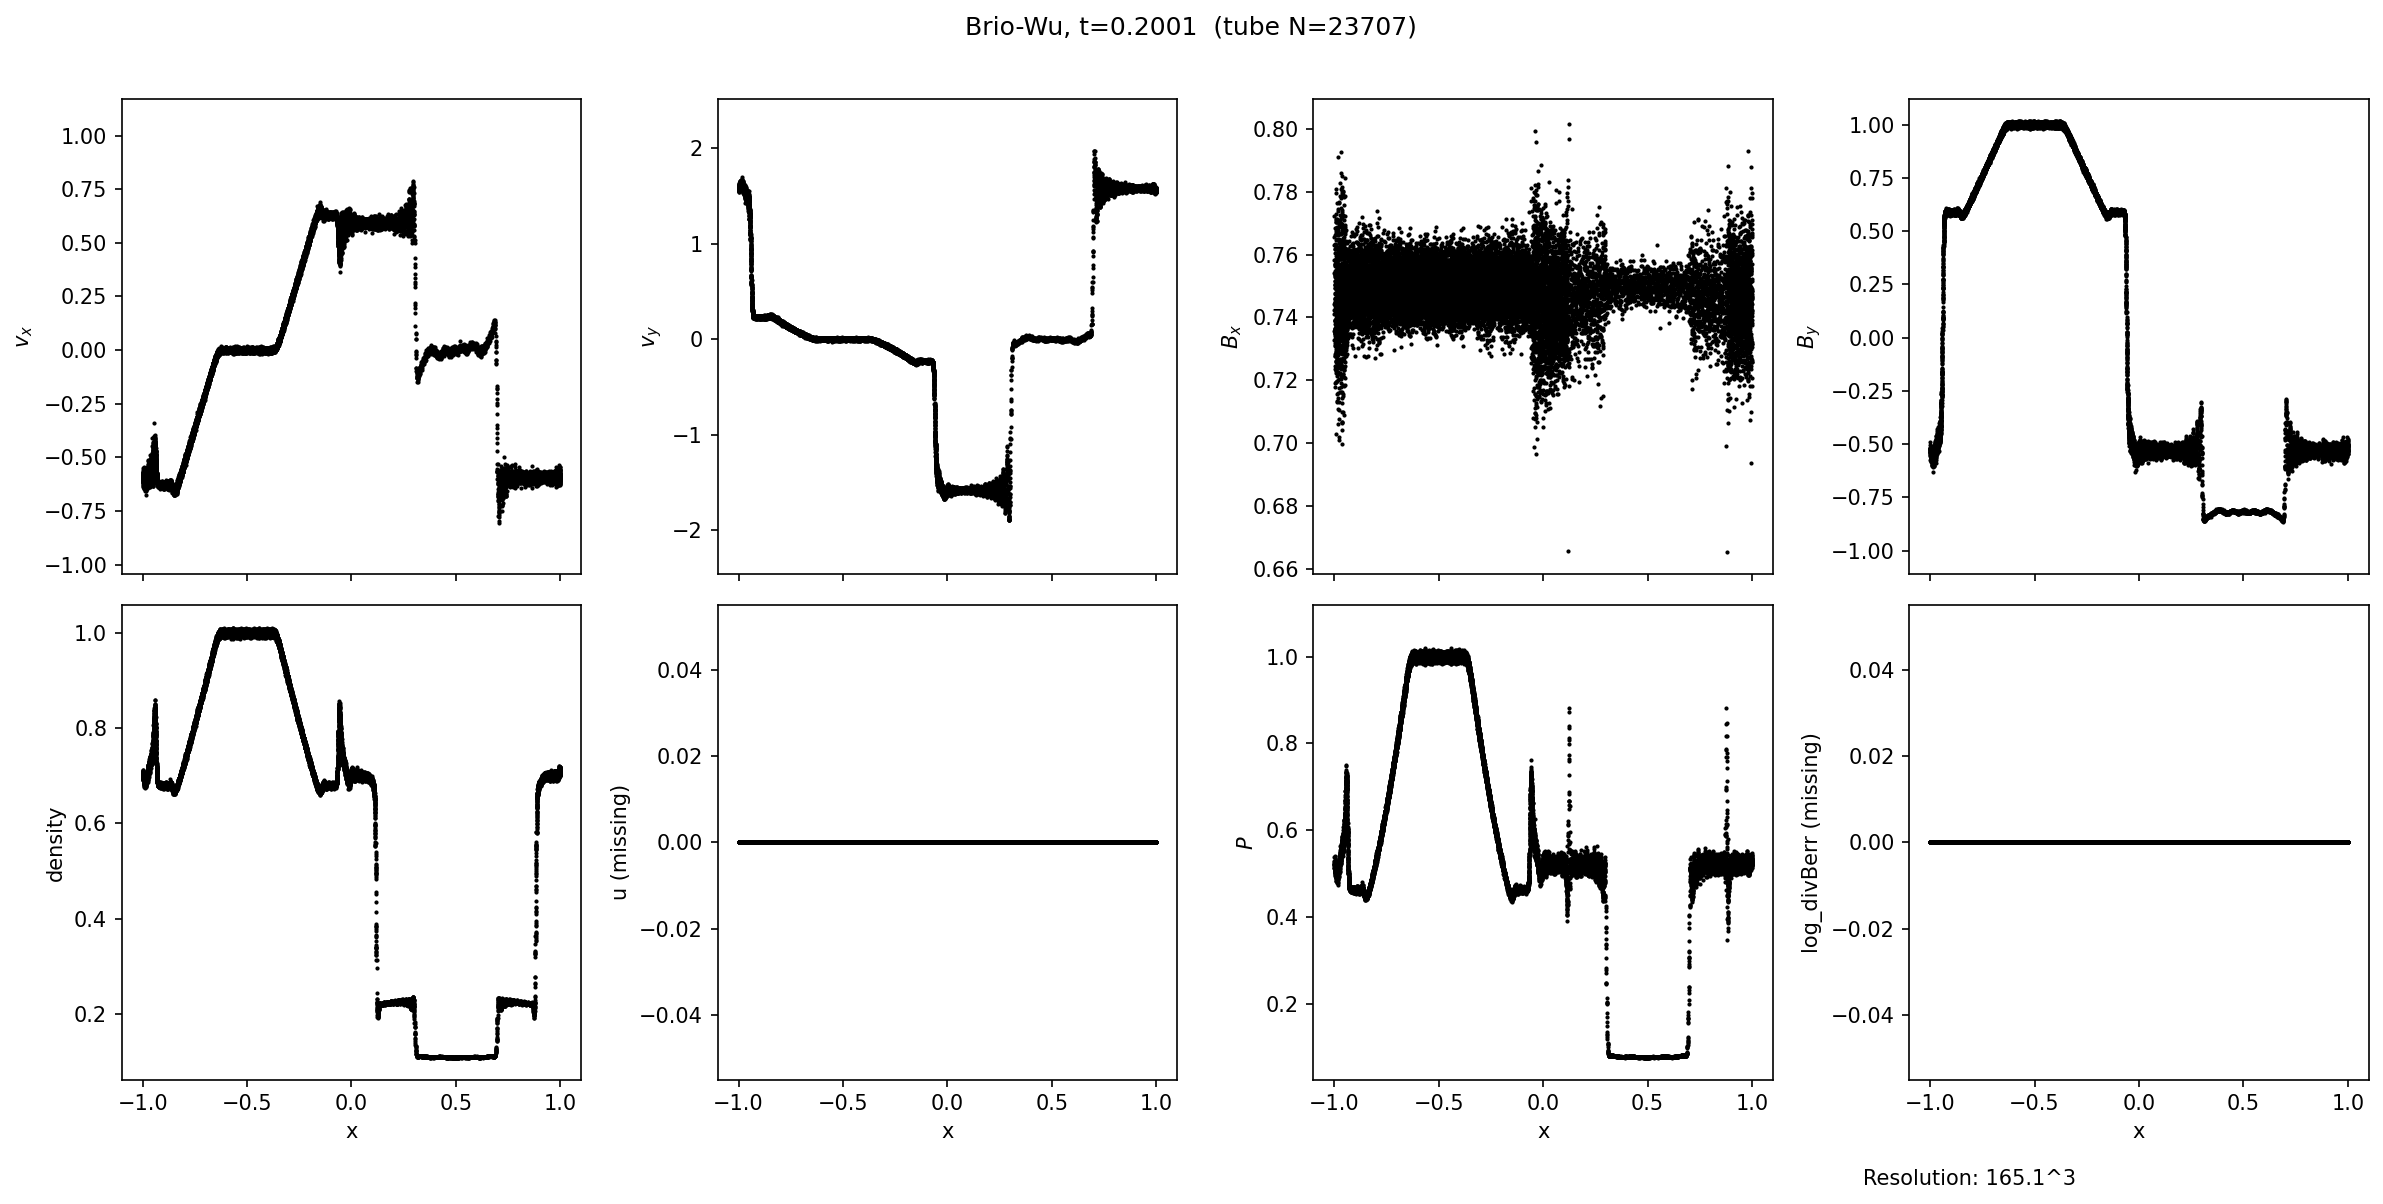
\includegraphics[width=0.8\linewidth]{img/Brio-Wu/shocktube_step2.png}
    \caption{Brio-Wu Shock Tube}
    \label{fig:placeholder}
\end{figure}

\begin{figure}
    \centering
    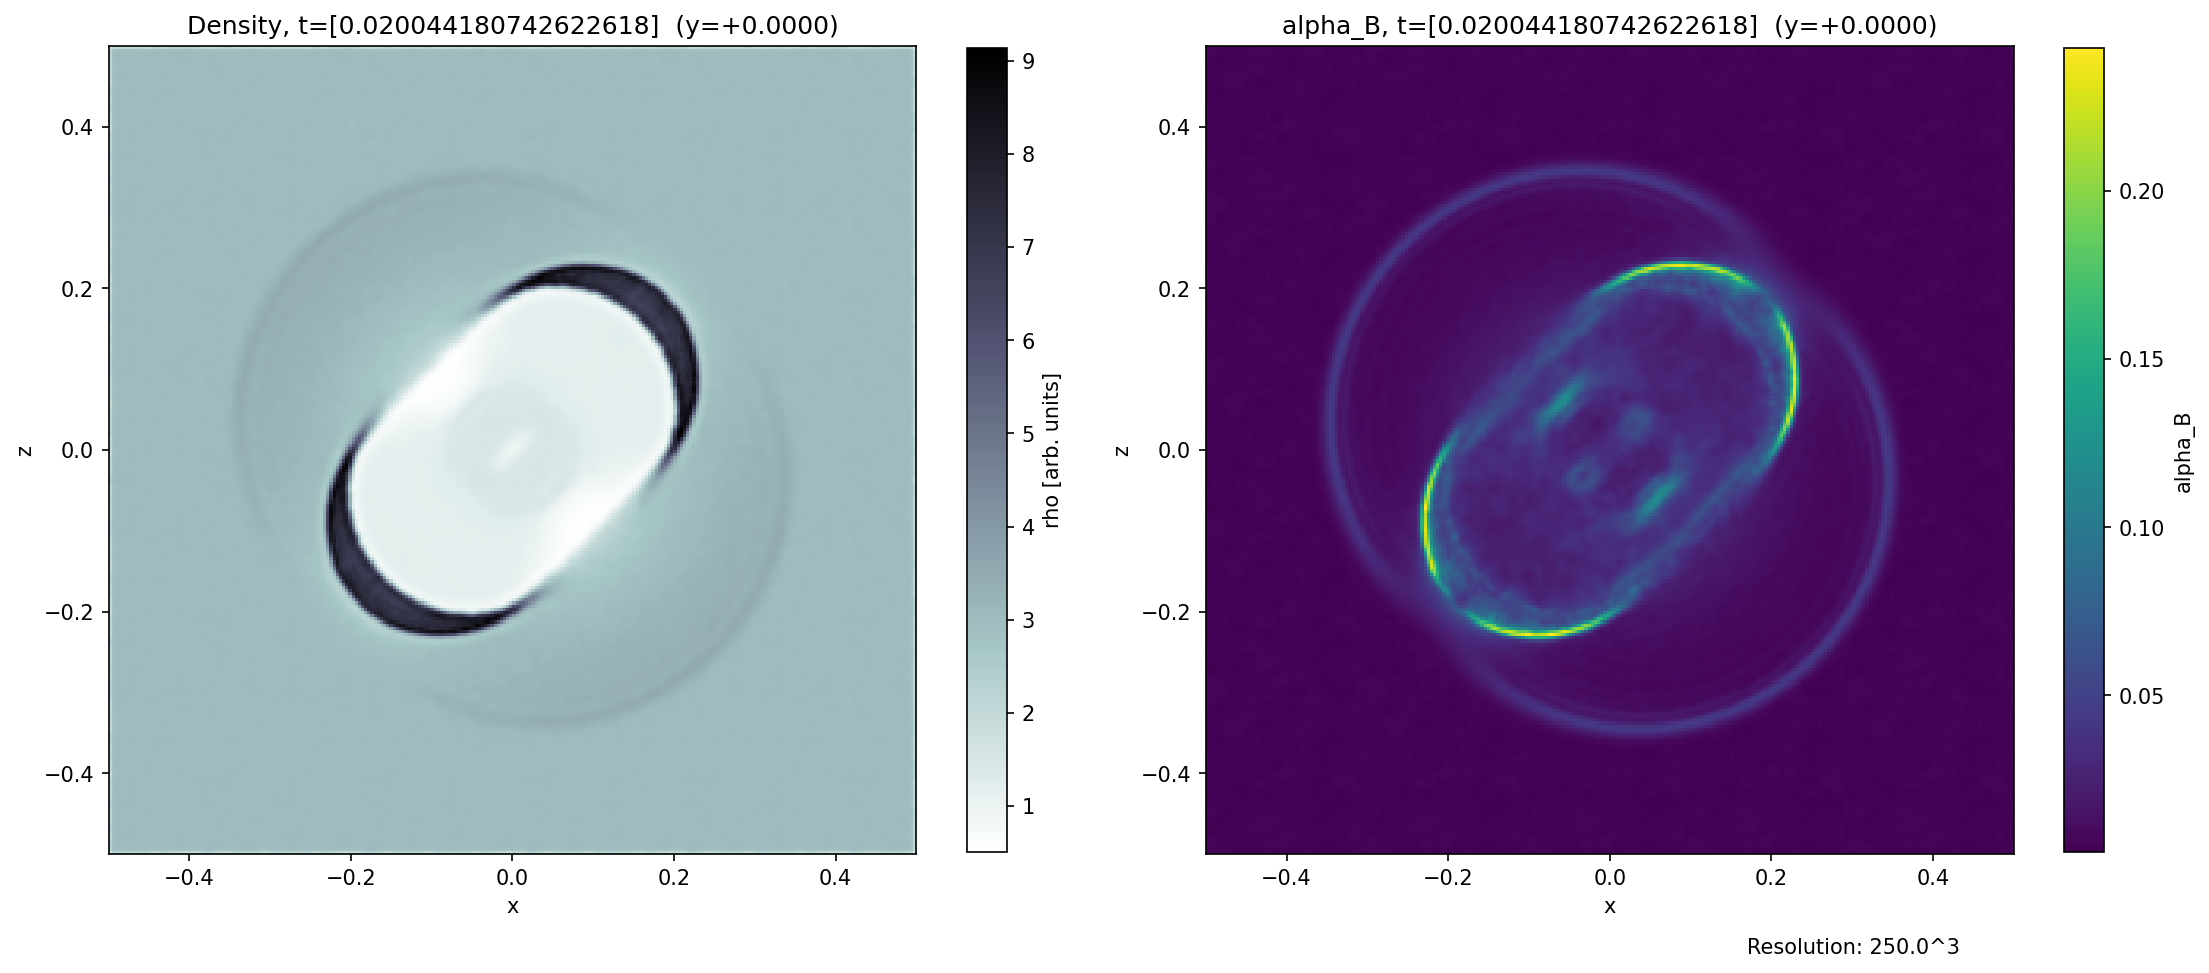
\includegraphics[width=0.8\linewidth]{img/sedov/slice_rho_step2_y+0.0000.png}
    \caption{Magnetic Sedov Blast}
    \label{fig:placeholder}
\end{figure}

\begin{figure}
    \centering
    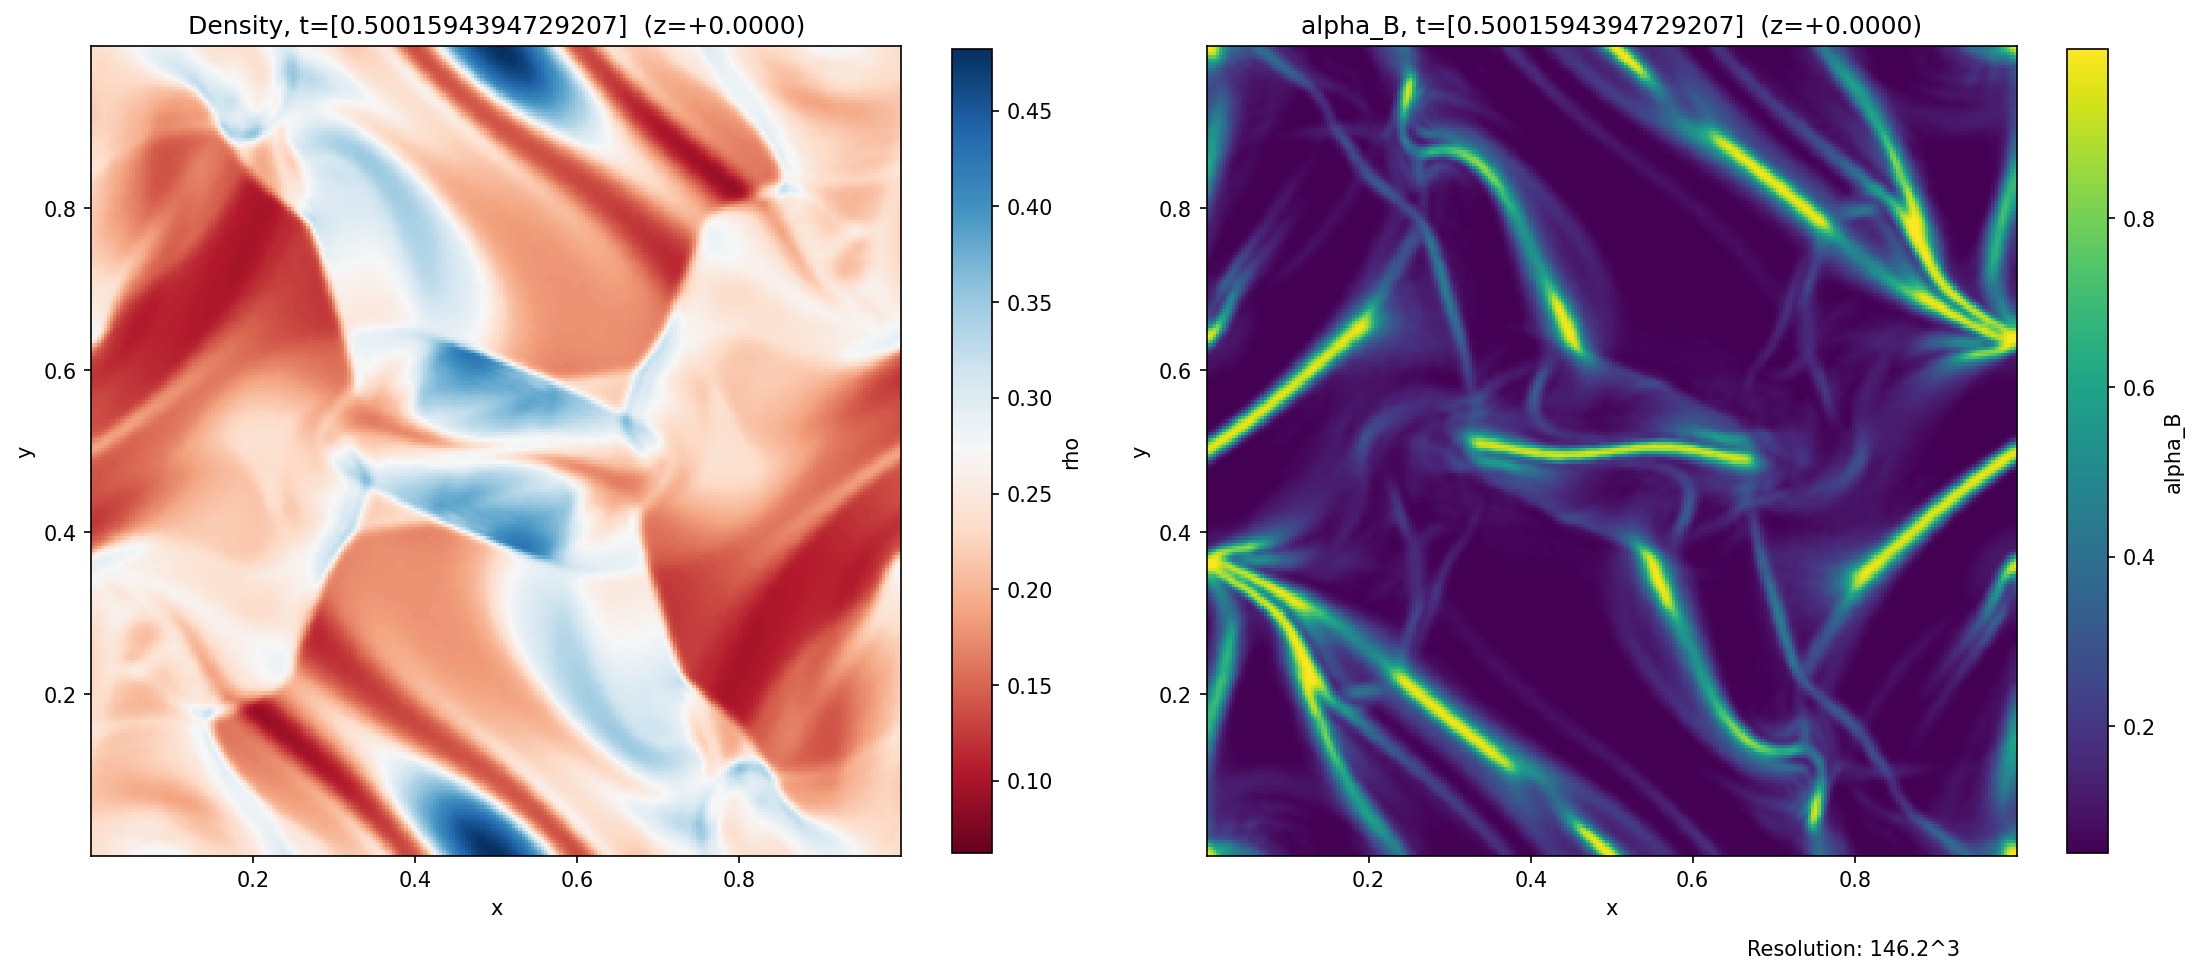
\includegraphics[width=0.8\linewidth]{img/OT_switch/slice_rho_step1_z+0.0000.png}
    \caption{Orszag-Tang Vortex}
    \label{fig:placeholder}
\end{figure}

\begin{figure}
    \centering
    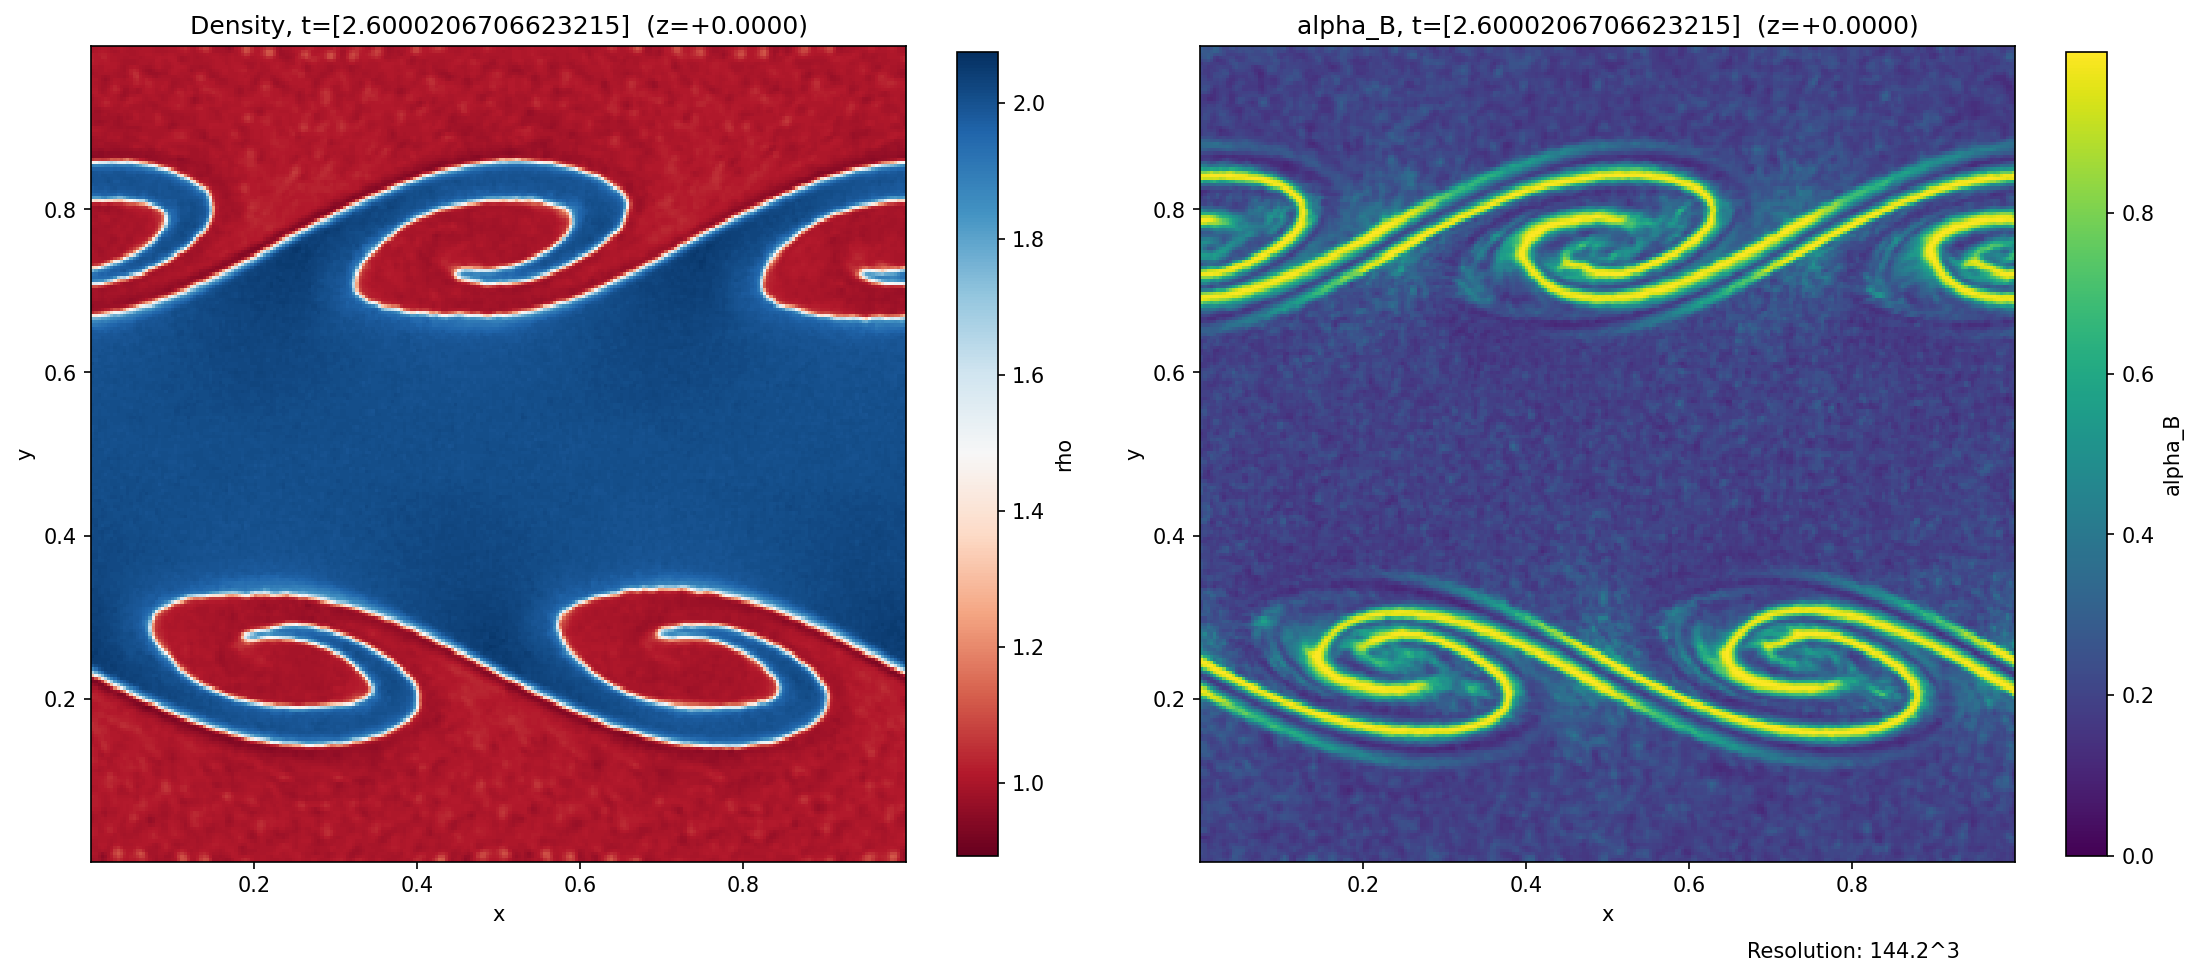
\includegraphics[width=0.8\linewidth]{img/KH/slice_rho_step3_z+0.0000.png}
    \caption{Kelvin-Helmholtz Instability}
    \label{fig:placeholder}
\end{figure}

\begin{figure}
    \centering
    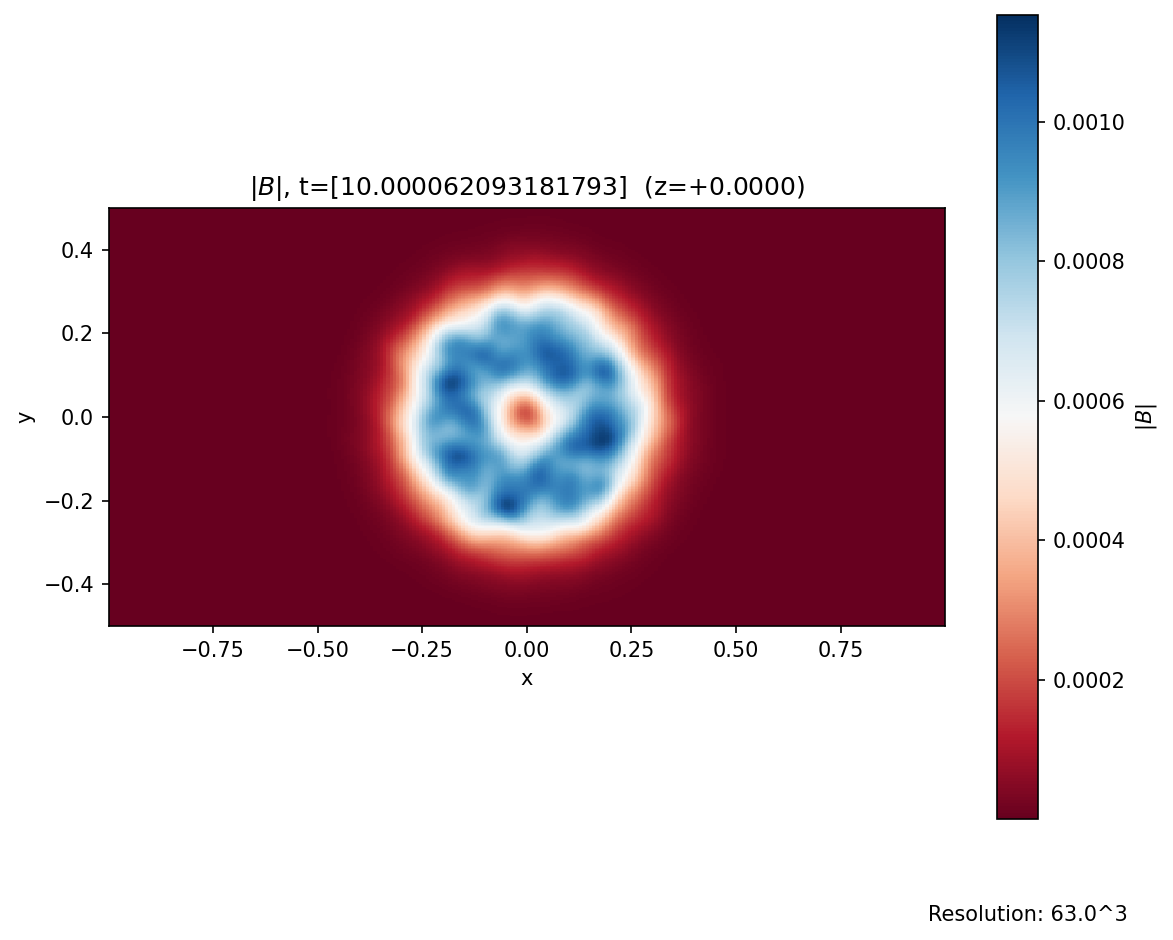
\includegraphics[width=0.5\linewidth]{img/MHD-Loop/slice_Bmag_step2_z+0.0000.png}
    \caption{MHD Advection Loop}
    \label{fig:placeholder}
\end{figure}

\begin{figure}
    \centering
    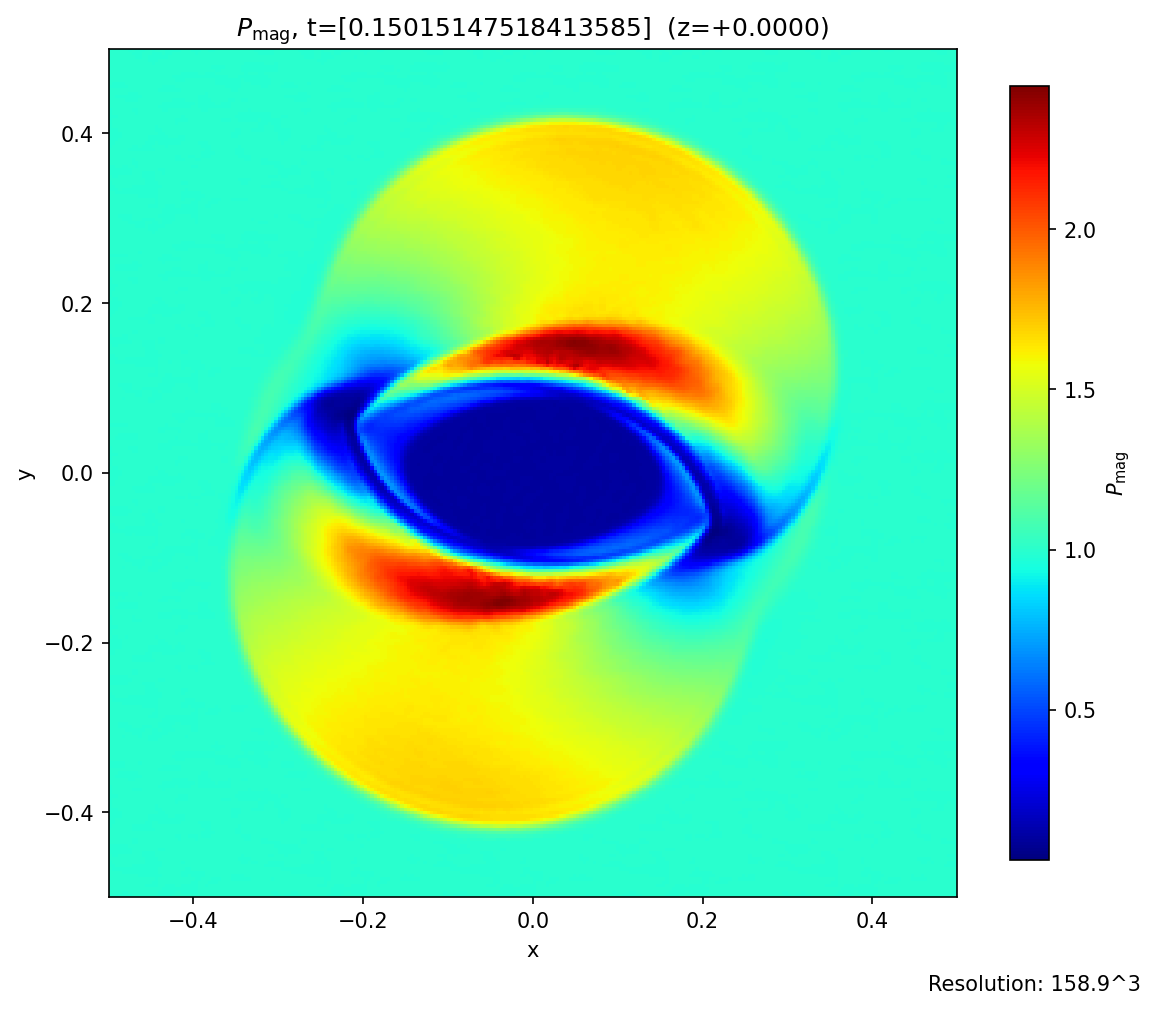
\includegraphics[width=0.45\linewidth]{img/Rotor/slice_Pmag_step0_z+0.0000.png}
    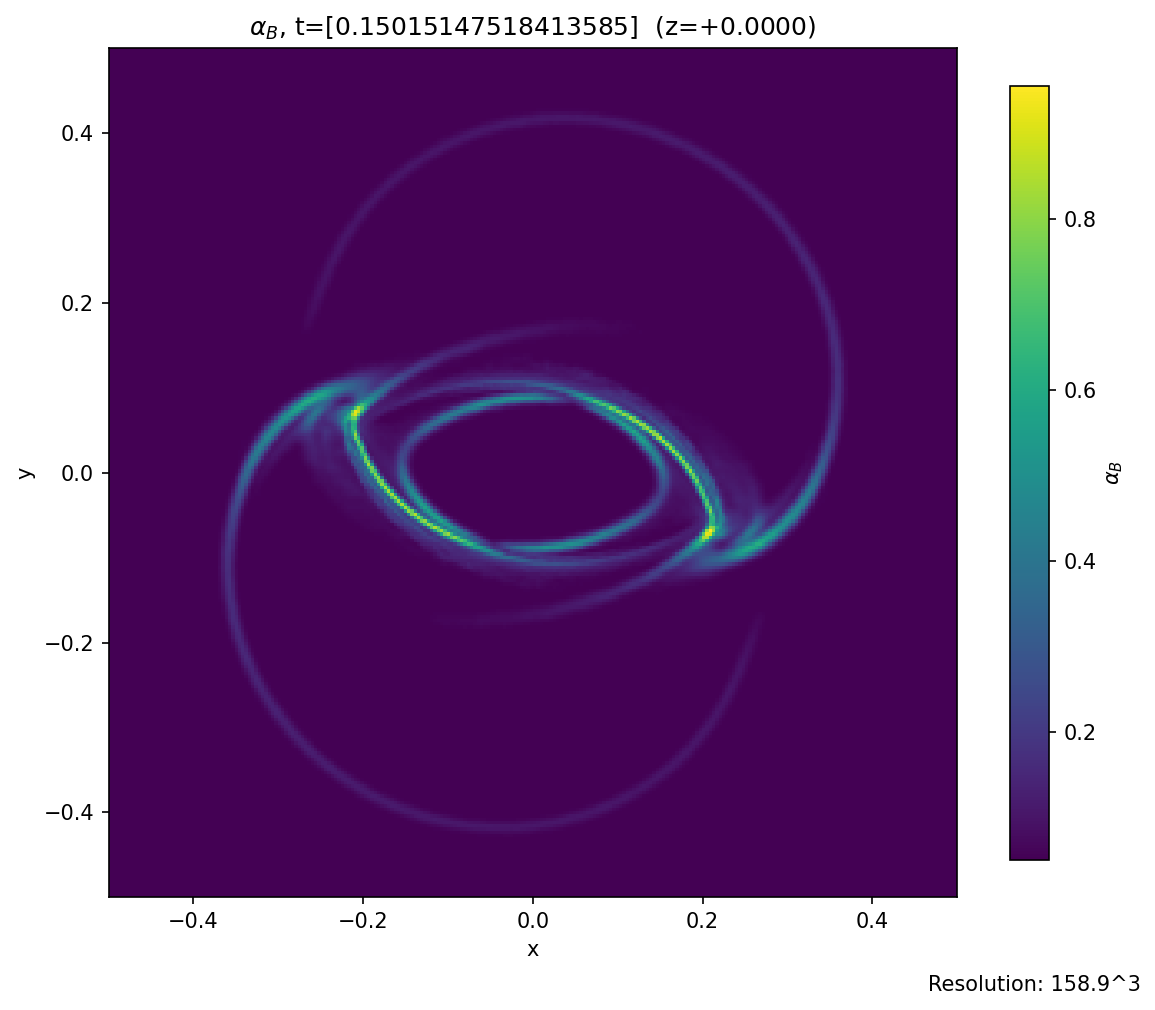
\includegraphics[width=0.45\linewidth]{img/Rotor/slice_alpha_B_step0_z+0.0000.png}
    \caption{MHD Rotor}
    \label{fig:placeholder}
\end{figure}